\documentclass[a4paper, 12pt]{article}
\usepackage{tikz}
\usetikzlibrary{positioning, arrows.meta, calc, shadows.blur}
\usepackage{xcolor}
\usepackage{colortbl}
\usepackage{float}
\usepackage{caption}
\usepackage{geometry}
\geometry{margin=1.5cm, landscape}

\definecolor{ehead}{RGB}{28,54,105}
\definecolor{epk}{RGB}{255,249,196}
\definecolor{efk}{RGB}{197,230,253}
\definecolor{ebg}{RGB}{245,248,252}

\newcommand{\tblpk}[2]{%
  \rowcolor{epk}{\scriptsize\ttfamily\bfseries #1} &
  {\scriptsize\ttfamily #2\;\textbf{\tiny PK}}\\[1pt]}
\newcommand{\tblfk}[2]{%
  \rowcolor{efk}{\scriptsize\ttfamily\itshape #1} &
  {\scriptsize\ttfamily #2\;{\tiny FK}}\\[1pt]}
\newcommand{\tblrow}[2]{%
  \rowcolor{ebg}{\scriptsize\ttfamily #1} &
  {\scriptsize\ttfamily #2}\\[1pt]}
\newcommand{\dbtbl}[2]{%
  \arrayrulecolor{ehead!50}%
  \begin{tabular}{@{\;}l@{\quad}l@{\;}}
    \multicolumn{2}{@{}c@{}}{%
      \cellcolor{ehead}\textcolor{white}%
      {\normalsize\bfseries\sffamily\;\;#1\;\;}}\\[0.5pt]
    \hline
    #2
    \hline
  \end{tabular}}

\begin{document}
\pagestyle{empty}

\begin{figure}[H]
\centering
{\large\bfseries\sffamily Figure 1: Entity Relationship Diagram --- Complete Database Schema}\\[4pt]
{\normalsize\sffamily Absolute grid placement (X, Y) to guarantee tables never overlap.}
\vspace{10pt}

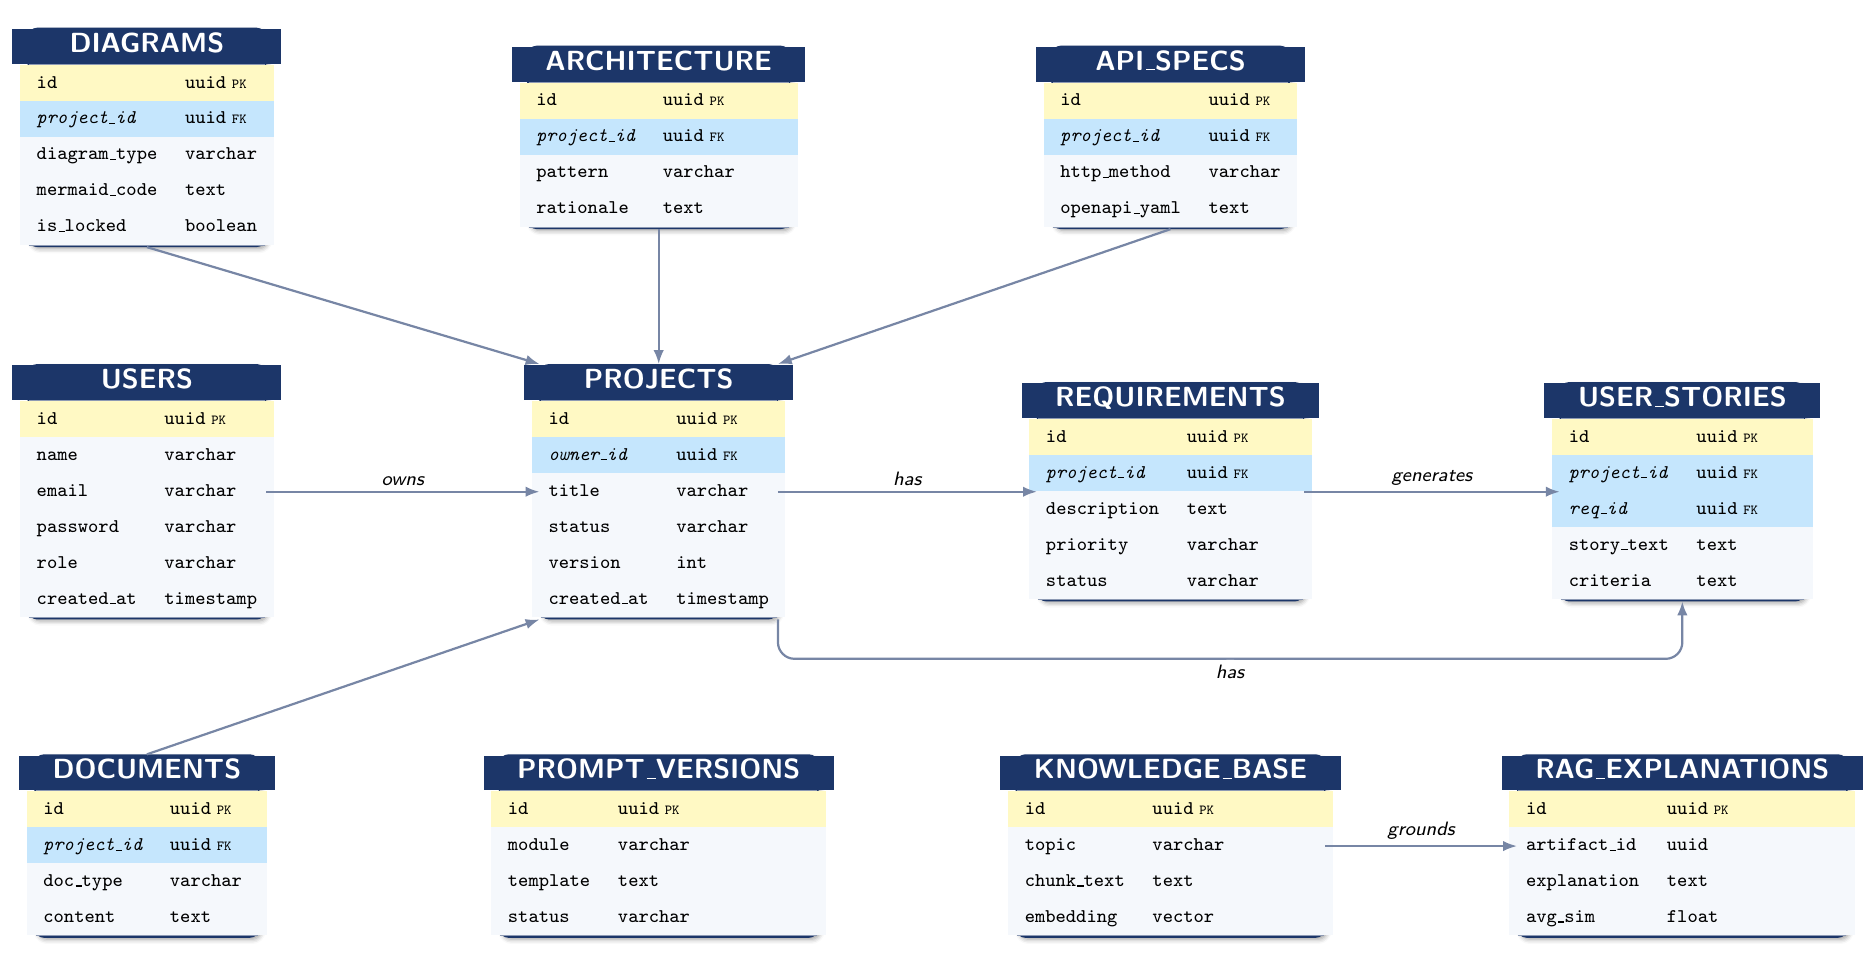
\begin{tikzpicture}[
  tbl/.style={draw=ehead, line width=1pt, inner sep=0pt,
              rounded corners=3pt,
              blur shadow={shadow blur steps=4,
                           shadow xshift=1pt, shadow yshift=-1pt}},
  arr/.style={draw=ehead!60, -{Latex[length=5pt]}, thick,
              rounded corners=6pt},
  lbl/.style={font=\scriptsize\sffamily\itshape, fill=white,
              inner sep=2pt}
]

% ==================== ABSOLUTE GRID PLACEMENT ====================
% Center Row (Y = 0)
\node[tbl] (users) at (-6.5, 0) {%
  \dbtbl{USERS}{
    \tblpk{id}{uuid}
    \tblrow{name}{varchar}
    \tblrow{email}{varchar}
    \tblrow{password}{varchar}
    \tblrow{role}{varchar}
    \tblrow{created\_at}{timestamp}
  }
};

\node[tbl] (projects) at (0, 0) {%
  \dbtbl{PROJECTS}{
    \tblpk{id}{uuid}
    \tblfk{owner\_id}{uuid}
    \tblrow{title}{varchar}
    \tblrow{status}{varchar}
    \tblrow{version}{int}
    \tblrow{created\_at}{timestamp}
  }
};

\node[tbl] (reqs) at (6.5, 0) {%
  \dbtbl{REQUIREMENTS}{
    \tblpk{id}{uuid}
    \tblfk{project\_id}{uuid}
    \tblrow{description}{text}
    \tblrow{priority}{varchar}
    \tblrow{status}{varchar}
  }
};

\node[tbl] (stories) at (13, 0) {%
  \dbtbl{USER\_STORIES}{
    \tblpk{id}{uuid}
    \tblfk{project\_id}{uuid}
    \tblfk{req\_id}{uuid}
    \tblrow{story\_text}{text}
    \tblrow{criteria}{text}
  }
};

% Top Row (Y = 4.5)
\node[tbl] (diagrams) at (-6.5, 4.5) {%
  \dbtbl{DIAGRAMS}{
    \tblpk{id}{uuid}
    \tblfk{project\_id}{uuid}
    \tblrow{diagram\_type}{varchar}
    \tblrow{mermaid\_code}{text}
    \tblrow{is\_locked}{boolean}
  }
};

\node[tbl] (arch) at (0, 4.5) {%
  \dbtbl{ARCHITECTURE}{
    \tblpk{id}{uuid}
    \tblfk{project\_id}{uuid}
    \tblrow{pattern}{varchar}
    \tblrow{rationale}{text}
  }
};

\node[tbl] (apispecs) at (6.5, 4.5) {%
  \dbtbl{API\_SPECS}{
    \tblpk{id}{uuid}
    \tblfk{project\_id}{uuid}
    \tblrow{http\_method}{varchar}
    \tblrow{openapi\_yaml}{text}
  }
};

% Bottom Row (Y = -4.5)
\node[tbl] (docs) at (-6.5, -4.5) {%
  \dbtbl{DOCUMENTS}{
    \tblpk{id}{uuid}
    \tblfk{project\_id}{uuid}
    \tblrow{doc\_type}{varchar}
    \tblrow{content}{text}
  }
};

\node[tbl] (prompts) at (0, -4.5) {%
  \dbtbl{PROMPT\_VERSIONS}{
    \tblpk{id}{uuid}
    \tblrow{module}{varchar}
    \tblrow{template}{text}
    \tblrow{status}{varchar}
  }
};

\node[tbl] (kb) at (6.5, -4.5) {%
  \dbtbl{KNOWLEDGE\_BASE}{
    \tblpk{id}{uuid}
    \tblrow{topic}{varchar}
    \tblrow{chunk\_text}{text}
    \tblrow{embedding}{vector}
  }
};

\node[tbl] (rag) at (13, -4.5) {%
  \dbtbl{RAG\_EXPLANATIONS}{
    \tblpk{id}{uuid}
    \tblrow{artifact\_id}{uuid}
    \tblrow{explanation}{text}
    \tblrow{avg\_sim}{float}
  }
};


% ==================== RELATIONSHIPS ====================
% Users to Projects
\draw[arr] (users.east) -- node[lbl, above]{owns} (projects.west);

% Top artifacts to Projects
\draw[arr] (diagrams.south) -- (projects.north west);
\draw[arr] (arch.south) -- (projects.north);
\draw[arr] (apispecs.south) -- (projects.north east);

% Bottom docs to Projects
\draw[arr] (docs.north) -- (projects.south west);

% Projects to Reqs & Stories
\draw[arr] (projects.east) -- node[lbl, above]{has} (reqs.west);
\draw[arr] (projects.south east) -- ++(0,-0.5) -| node[lbl, pos=0.25, below]{has} (stories.south);

% Reqs to Stories
\draw[arr] (reqs.east) -- node[lbl, above]{generates} (stories.west);

% KB to RAG
\draw[arr] (kb.east) -- node[lbl, above]{grounds} (rag.west);

\end{tikzpicture}
\end{figure}

\end{document}
